\section{Experimental results}

\subsection{The single Fano cavity}

Figures:
\begin{itemize}
    \item Single fano cavity transmission as a function of wavelength.
    \item Short scan of the single fano cavity tranmission, with found linewidth.
    \item Long scan Fabry-Perot fringes for determining FSR -> cavity length. 
    \item linewidth as a function of cavity length (compare with broadban cavity).
\end{itemize}

\begin{figure}[h!]
    \centering
    \begin{subfigure}[b]{0.49\textwidth}
        \centering
        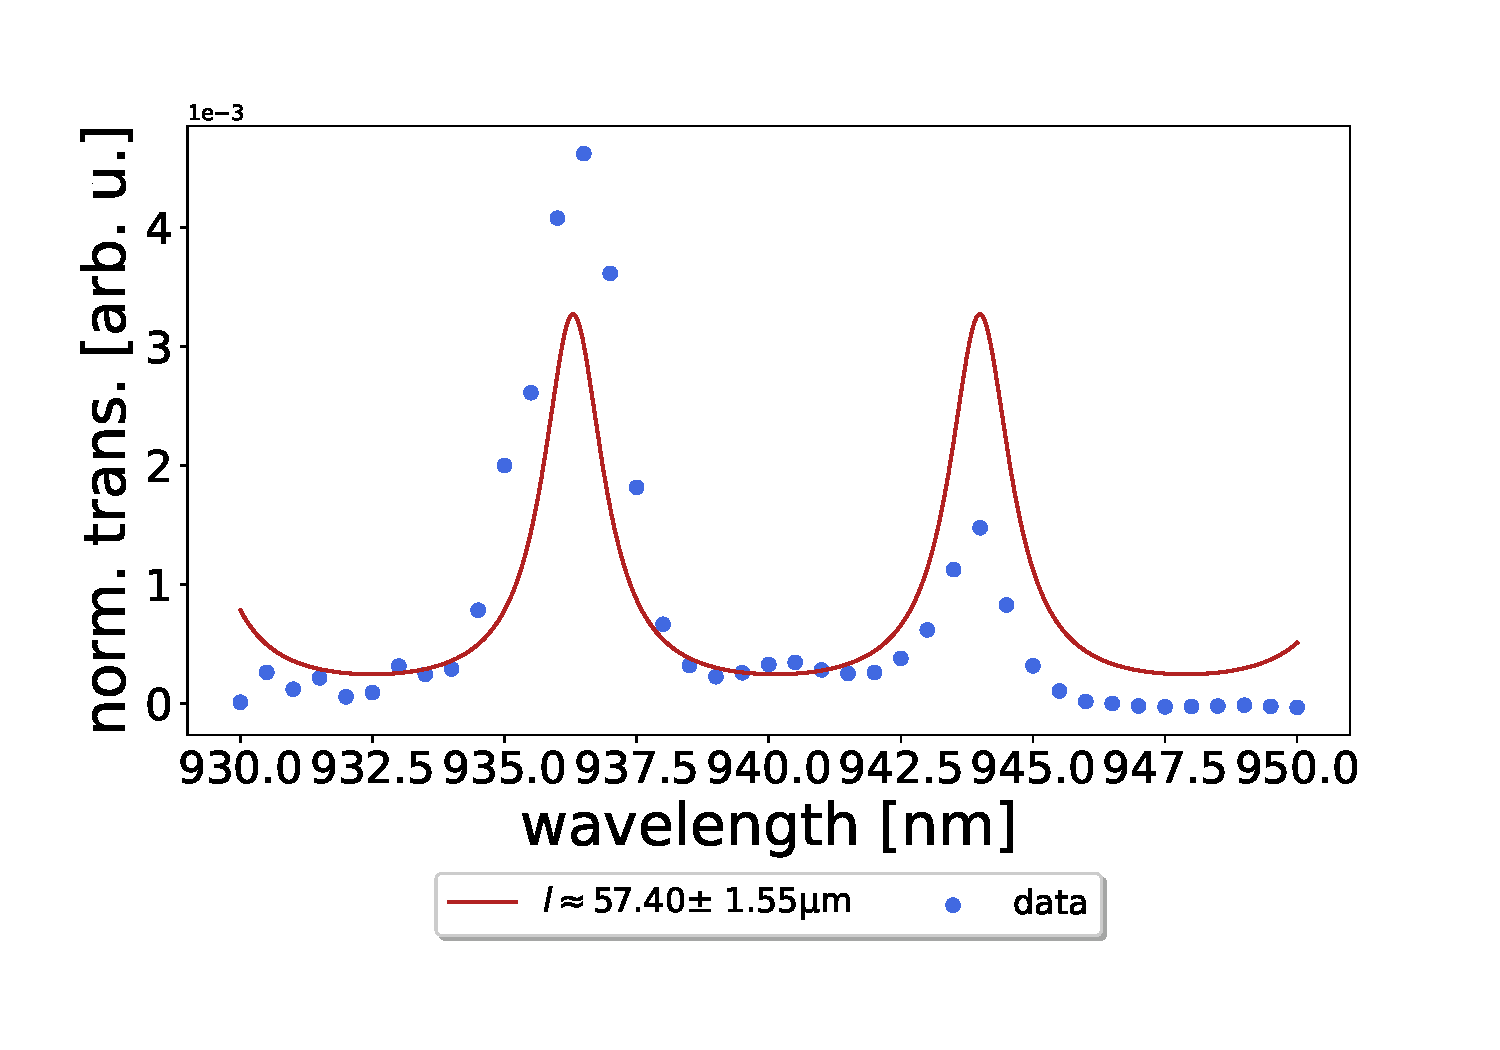
\includegraphics[width=\textwidth]{figures/results/60um_M5_FSR_fit.pdf}
        \caption{}
        \label{fig:short_single_fano_FSR}
    \end{subfigure}
    \begin{subfigure}[b]{0.49\textwidth}
        \centering
        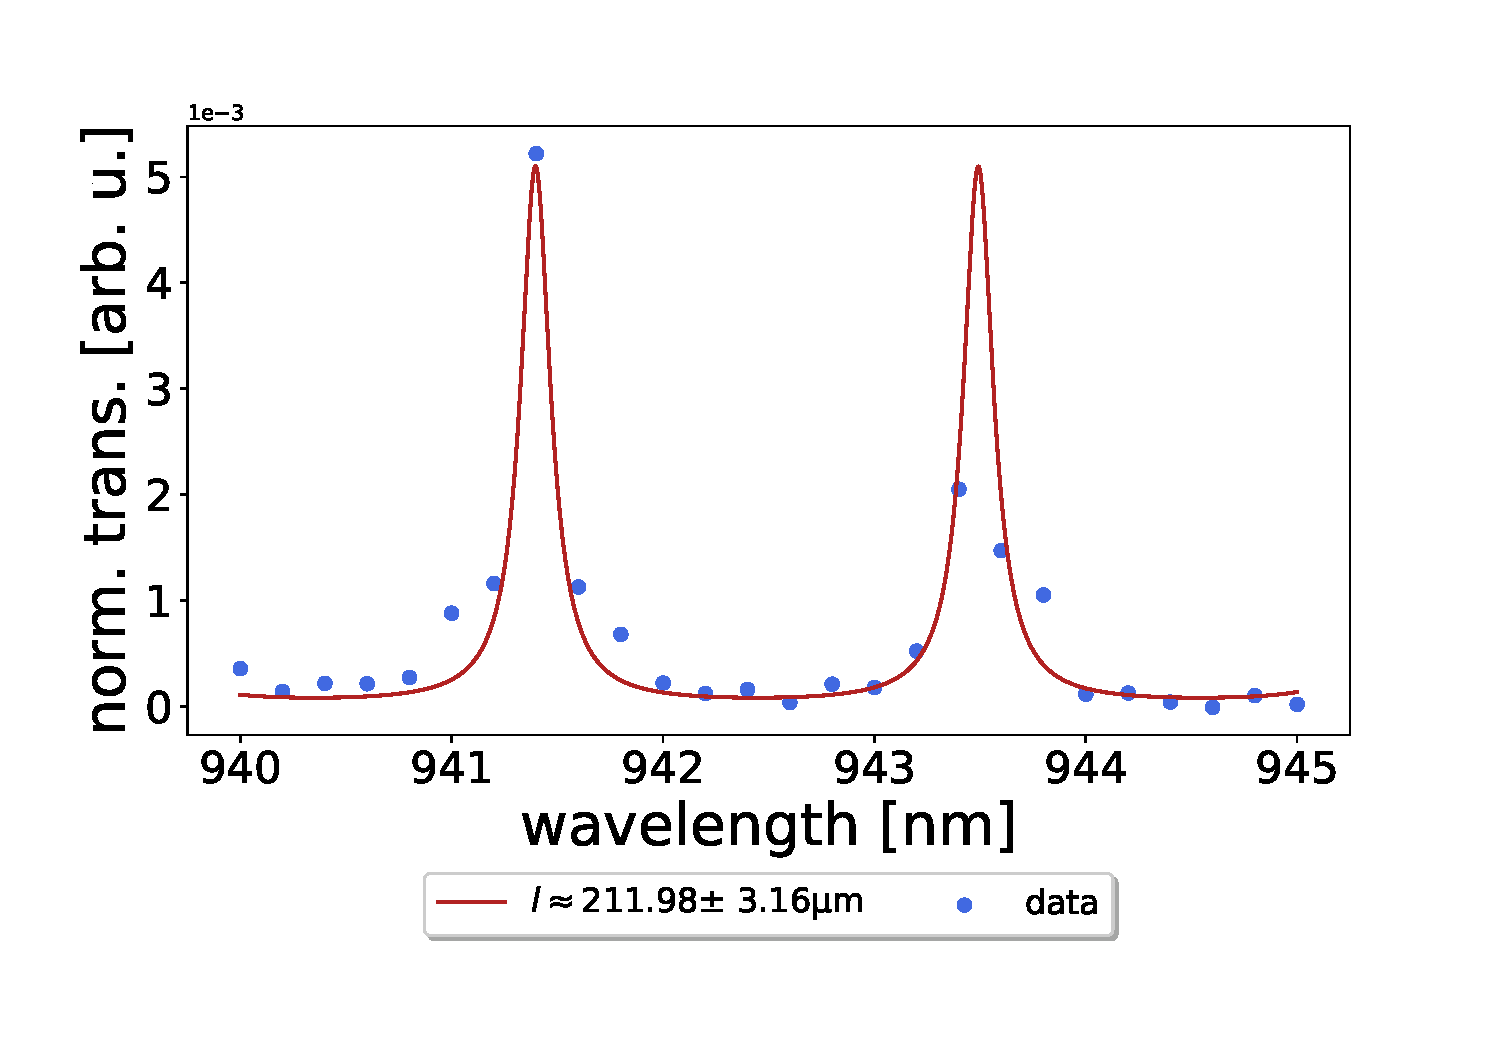
\includegraphics[width=\textwidth]{figures/results/220um_M5_FSR_fit.pdf}
        \caption{}
        \label{fig:long_single_fano_FSR}
    \end{subfigure}
\end{figure}

\begin{figure}[h!]
    \centering
    \begin{subfigure}[b]{0.49\textwidth}
        \centering
        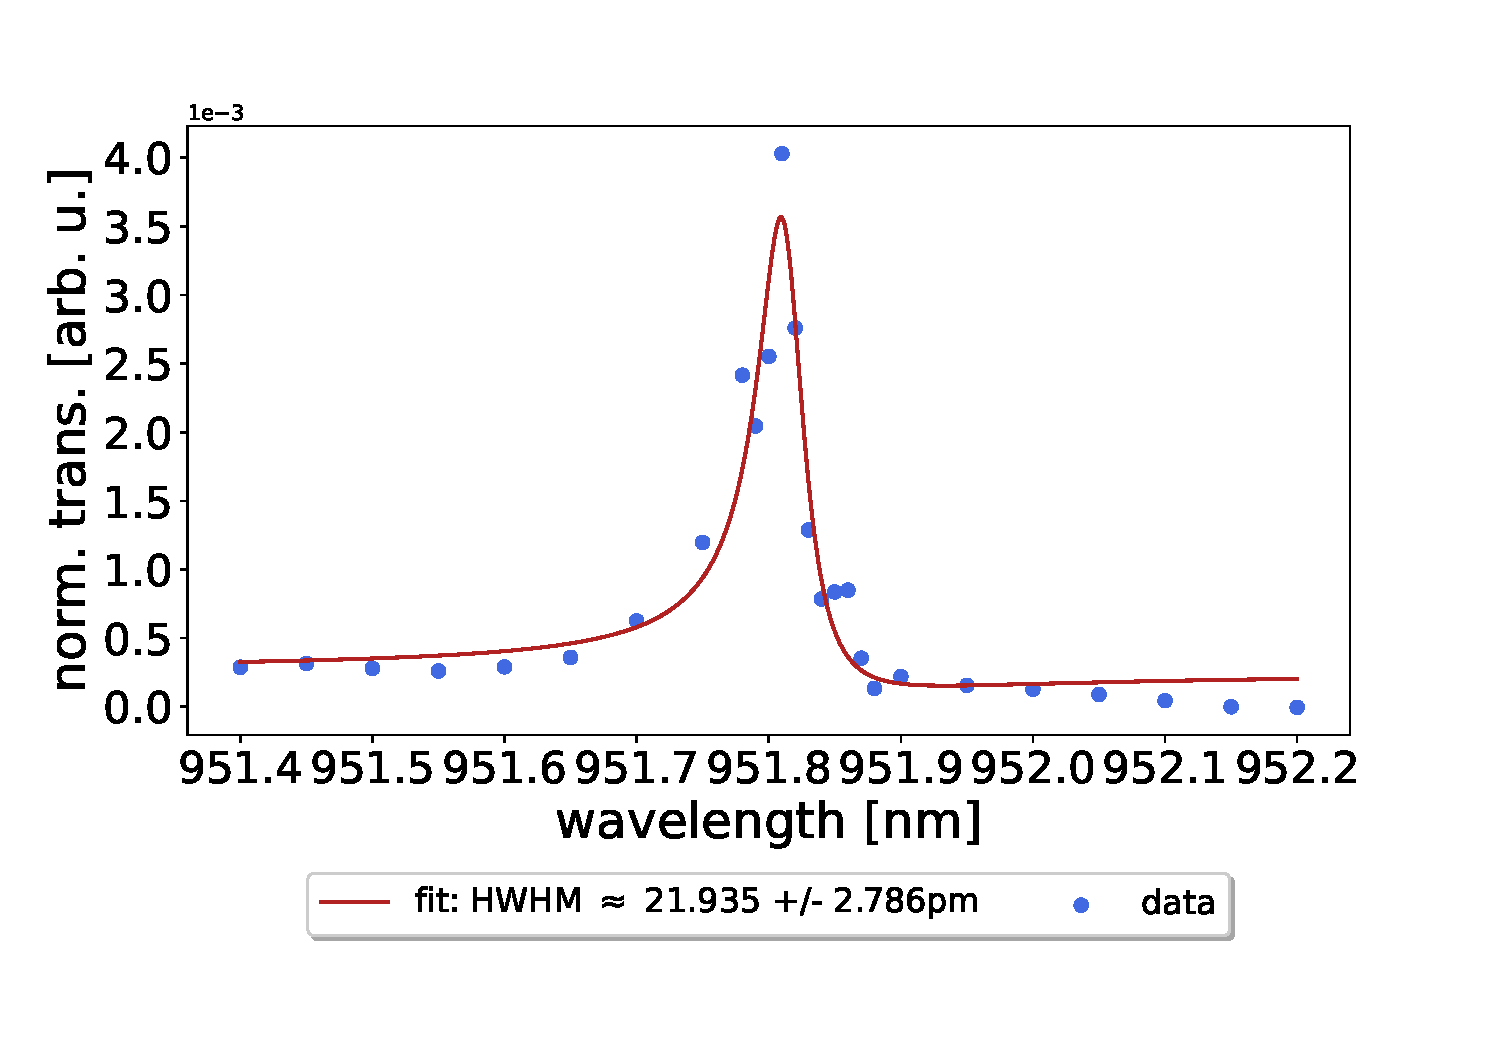
\includegraphics[width=\textwidth]{figures/results/60um_M5_fit_1.pdf}
        \caption{}
        \label{fig:short_single_fano_trans}
    \end{subfigure}
    \begin{subfigure}[b]{0.49\textwidth}
        \centering
        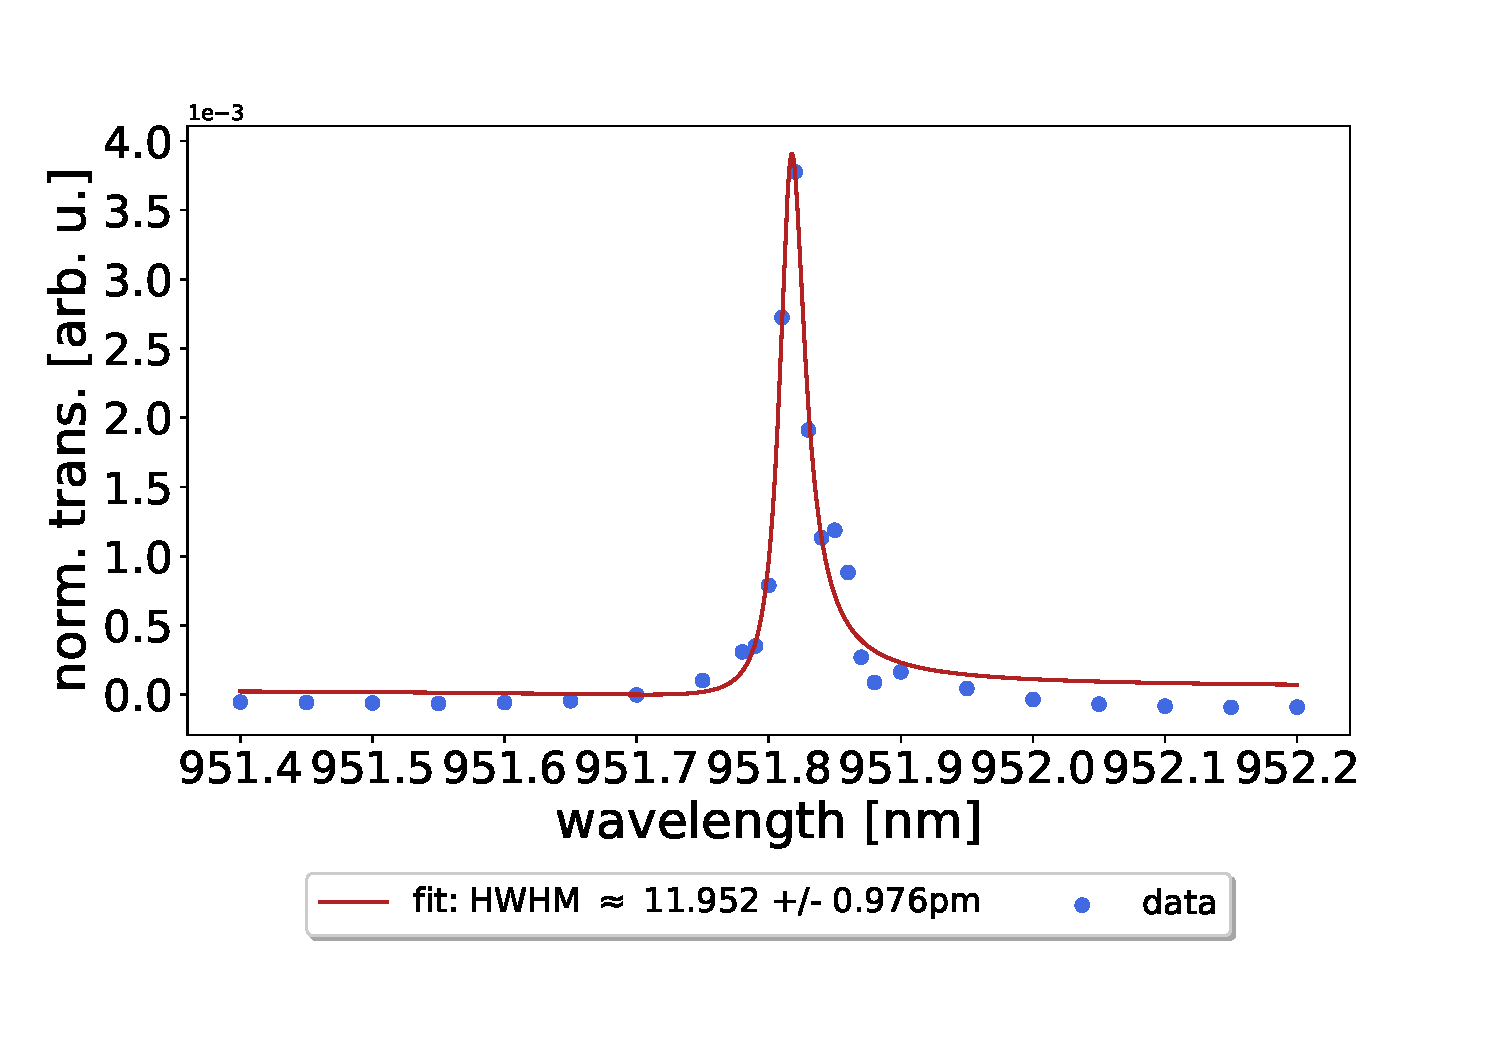
\includegraphics[width=\textwidth]{figures/results/220um_M5_fit_4.pdf}
        \caption{}
        \label{fig:long_single_fano_trans}
    \end{subfigure}
\end{figure}

\begin{figure}[h!]
    \centering
    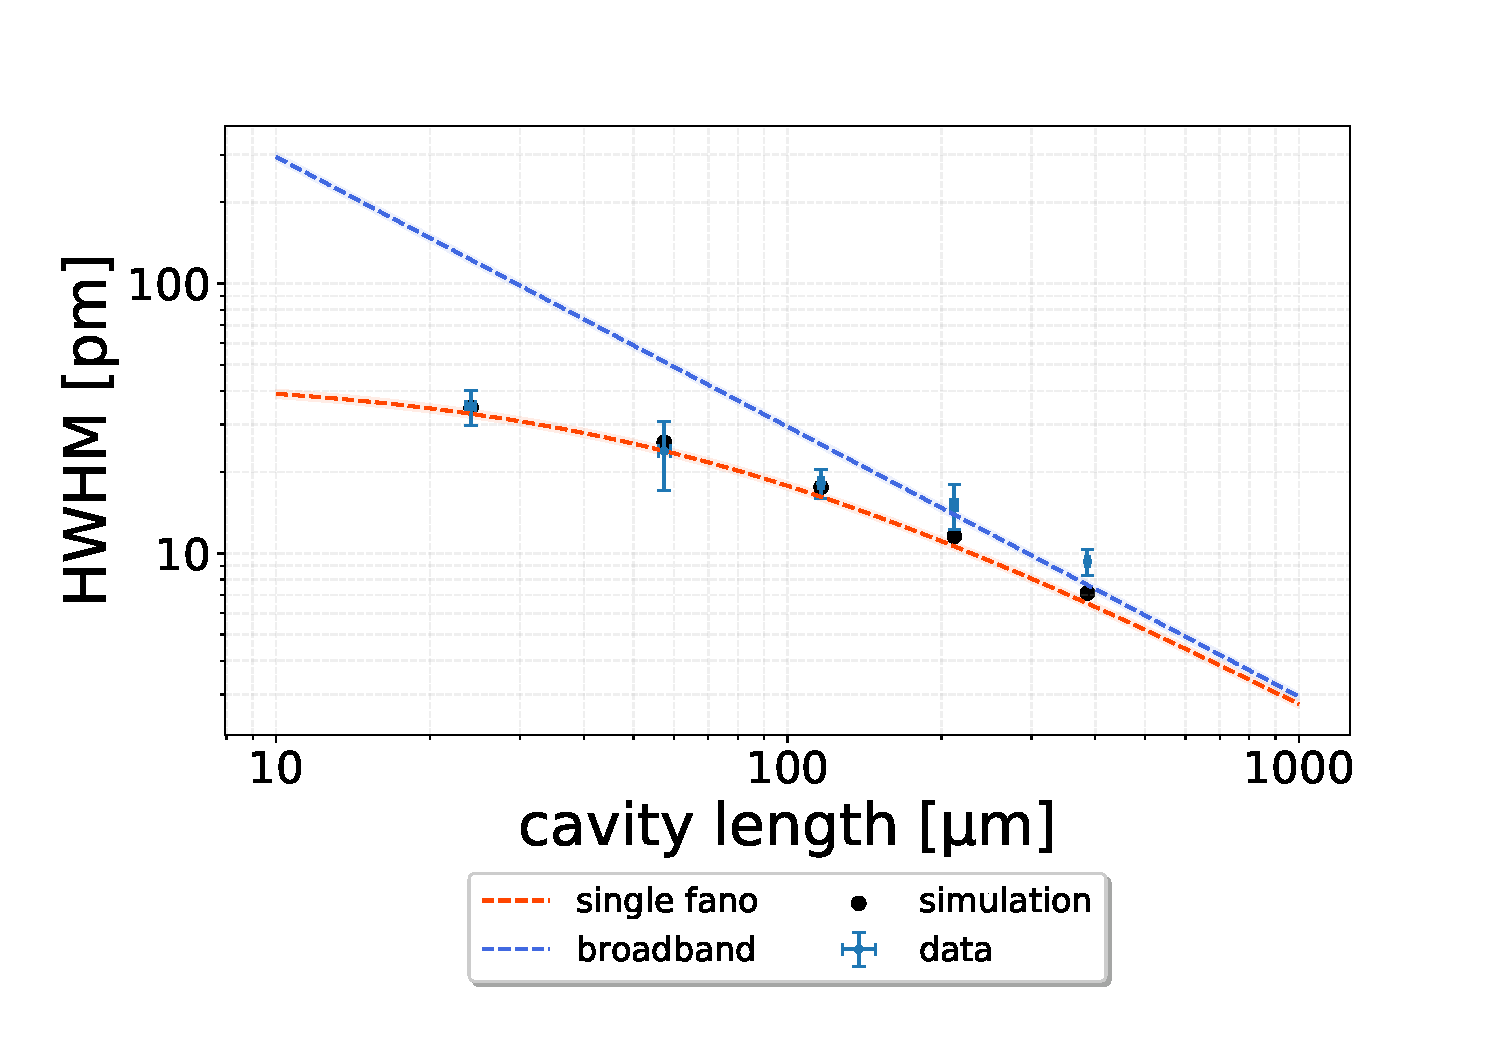
\includegraphics[width=0.7\textwidth]{figures/results/HWHM_vs_cavity_length_single_fano.pdf}
    \caption{}
    \label{fig:HWHM_vs_time_single_fano_data}
\end{figure}

\subsection{The double Fano cavity}

\subsubsection{Realizing the double fano model}

Figures: 
\begin{itemize}
    \item Fit of the double fano model (long + short cavity)
\end{itemize}

\begin{figure}[h!]
    \centering
    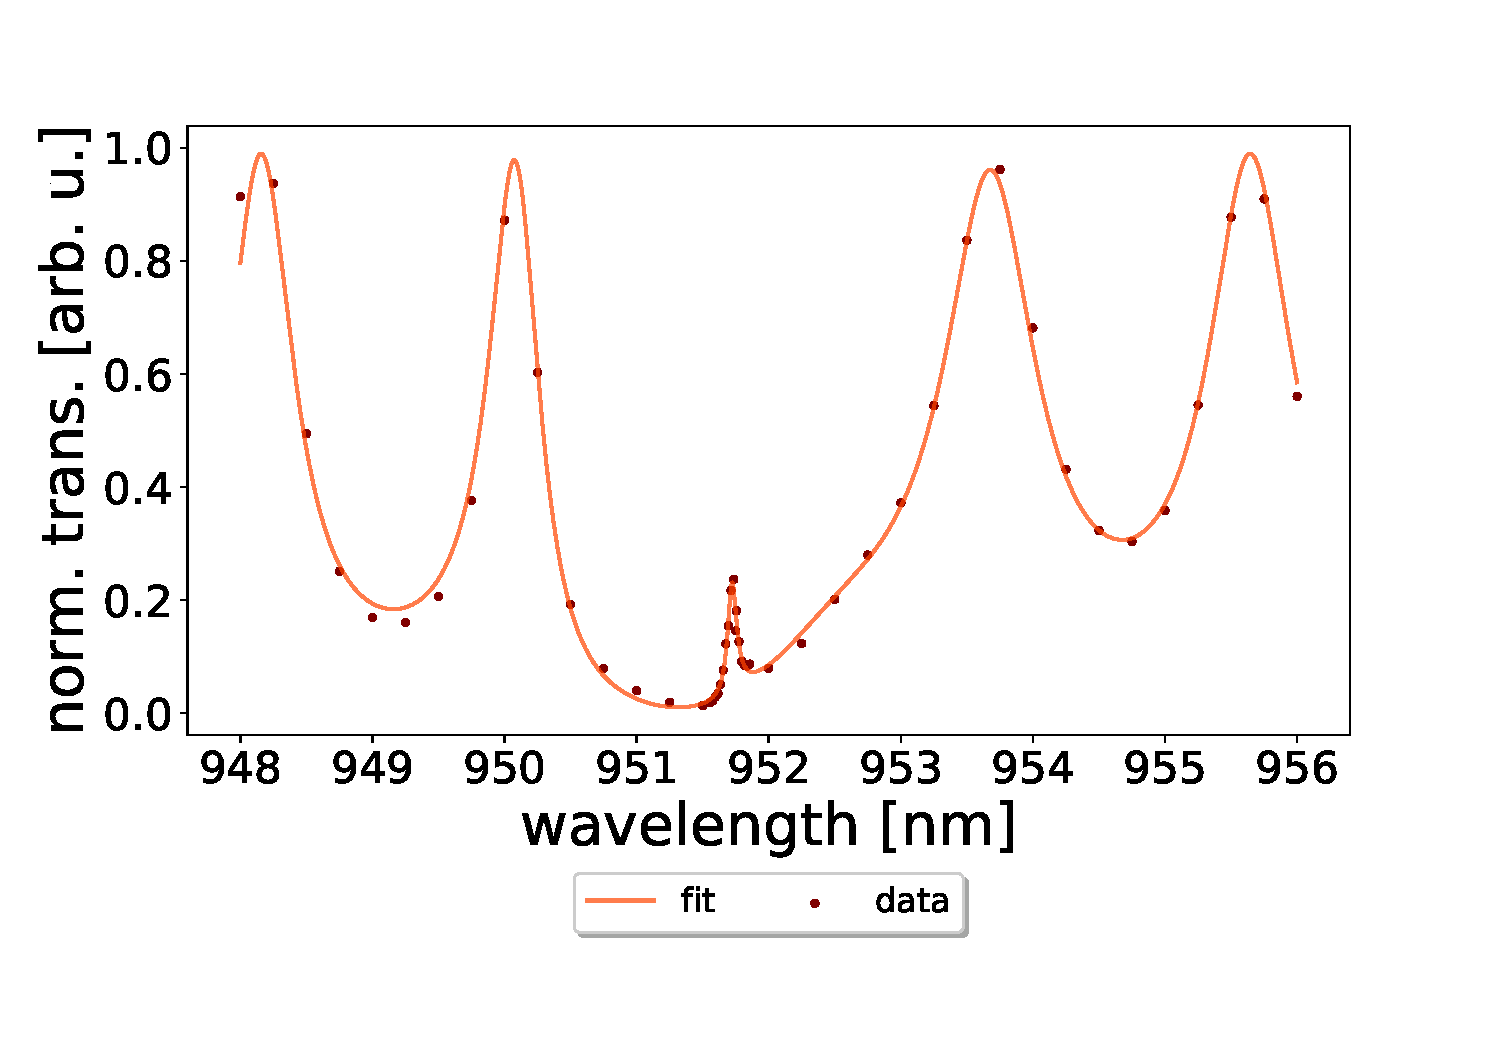
\includegraphics[width=0.7\textwidth]{figures/results/238um_long_scan_fit.pdf}
    \caption{G1: 
    $\lambda$0 =  951.3701127680025 nm 
    $\lambda$1 =  951.4030662431192 nm 
    td =  0.6987494932161454 
    $\gamma \lambda$ =  0.7571474313977703 nm 
    $\alpha$ =  -4.941261358750405e-08
    G2: 
    $\lambda$0 =  951.6390536402713 nm 
    $\lambda$1 =  951.7701388562424 nm 
    td =  0.8980584603164458 
    $\gamma \lambda$ =  0.5091431173169724 nm 
    $\alpha$ =  8.513254832146483e-07
    cavity length:  238925.73648797692 $\mu$m
    losses:  0.2032944039987356}
    \label{fig:238um_long_scan_fit}
\end{figure}

\begin{figure}[h!]
    \centering
    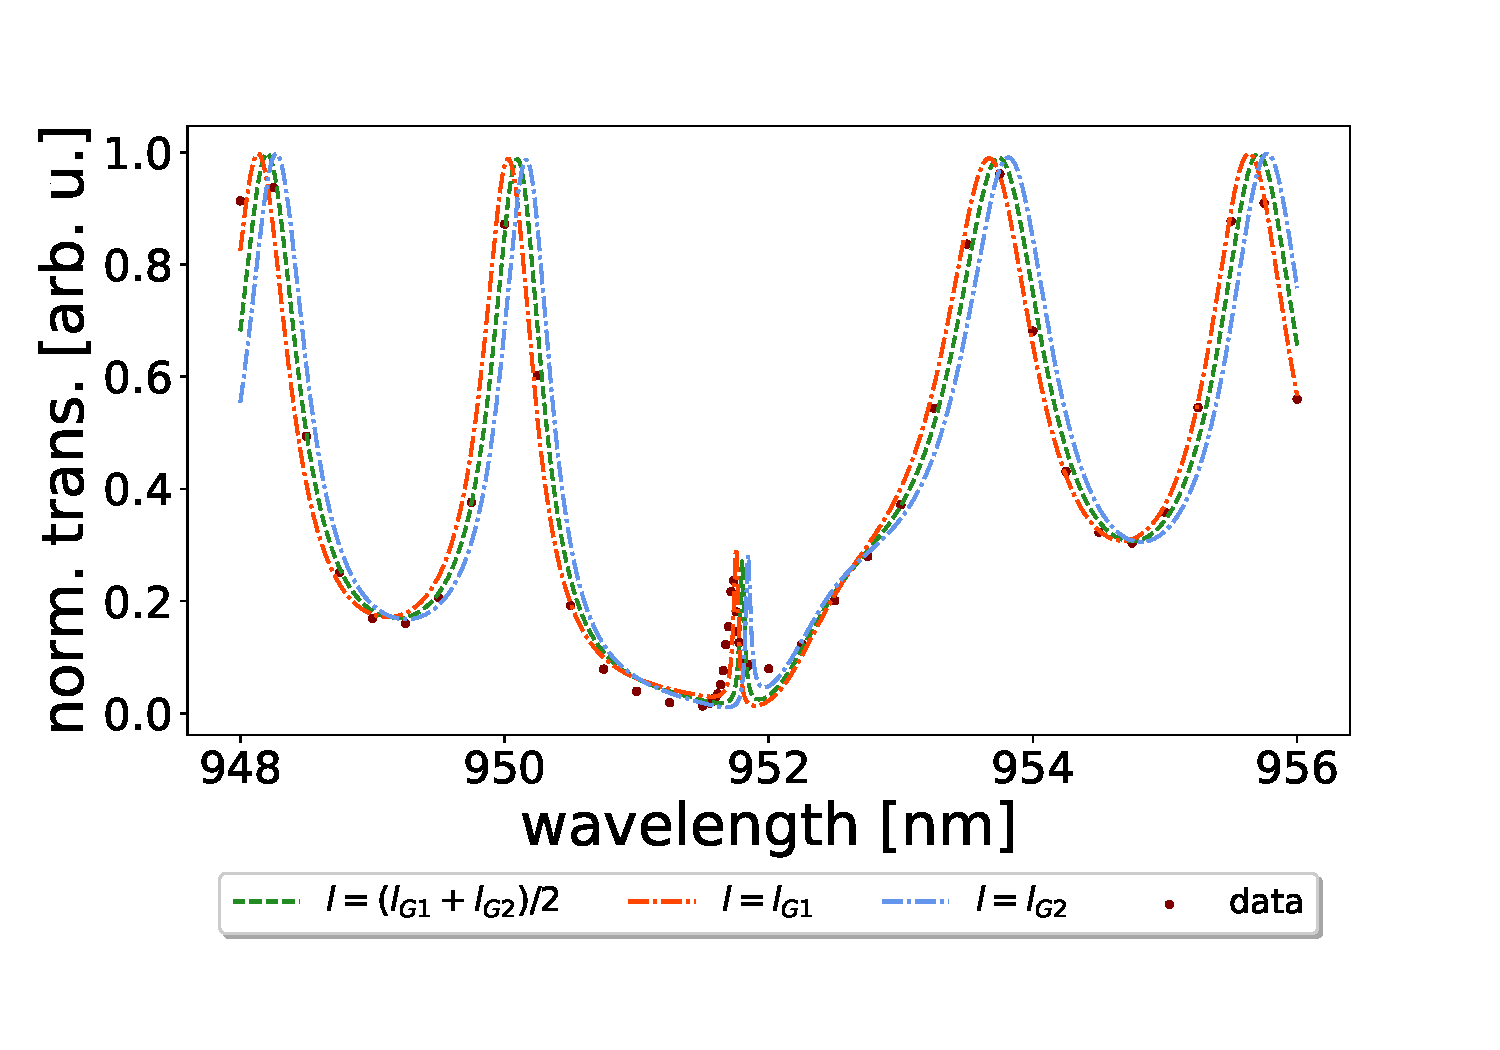
\includegraphics[width=0.7\textwidth]{figures/results/238um_long_scan_sim_comparison.pdf}
    \caption{$l_{G1} = 239.3975 \mu m$, $l_{G2} = 239.4317 \mu m$, $(l_{G1} + l_{G2})/2 = 239.4146 \mu m$}
    \label{fig:238um_long_scan_sim_comparison}
\end{figure}

\begin{figure}[h!]
    \centering
    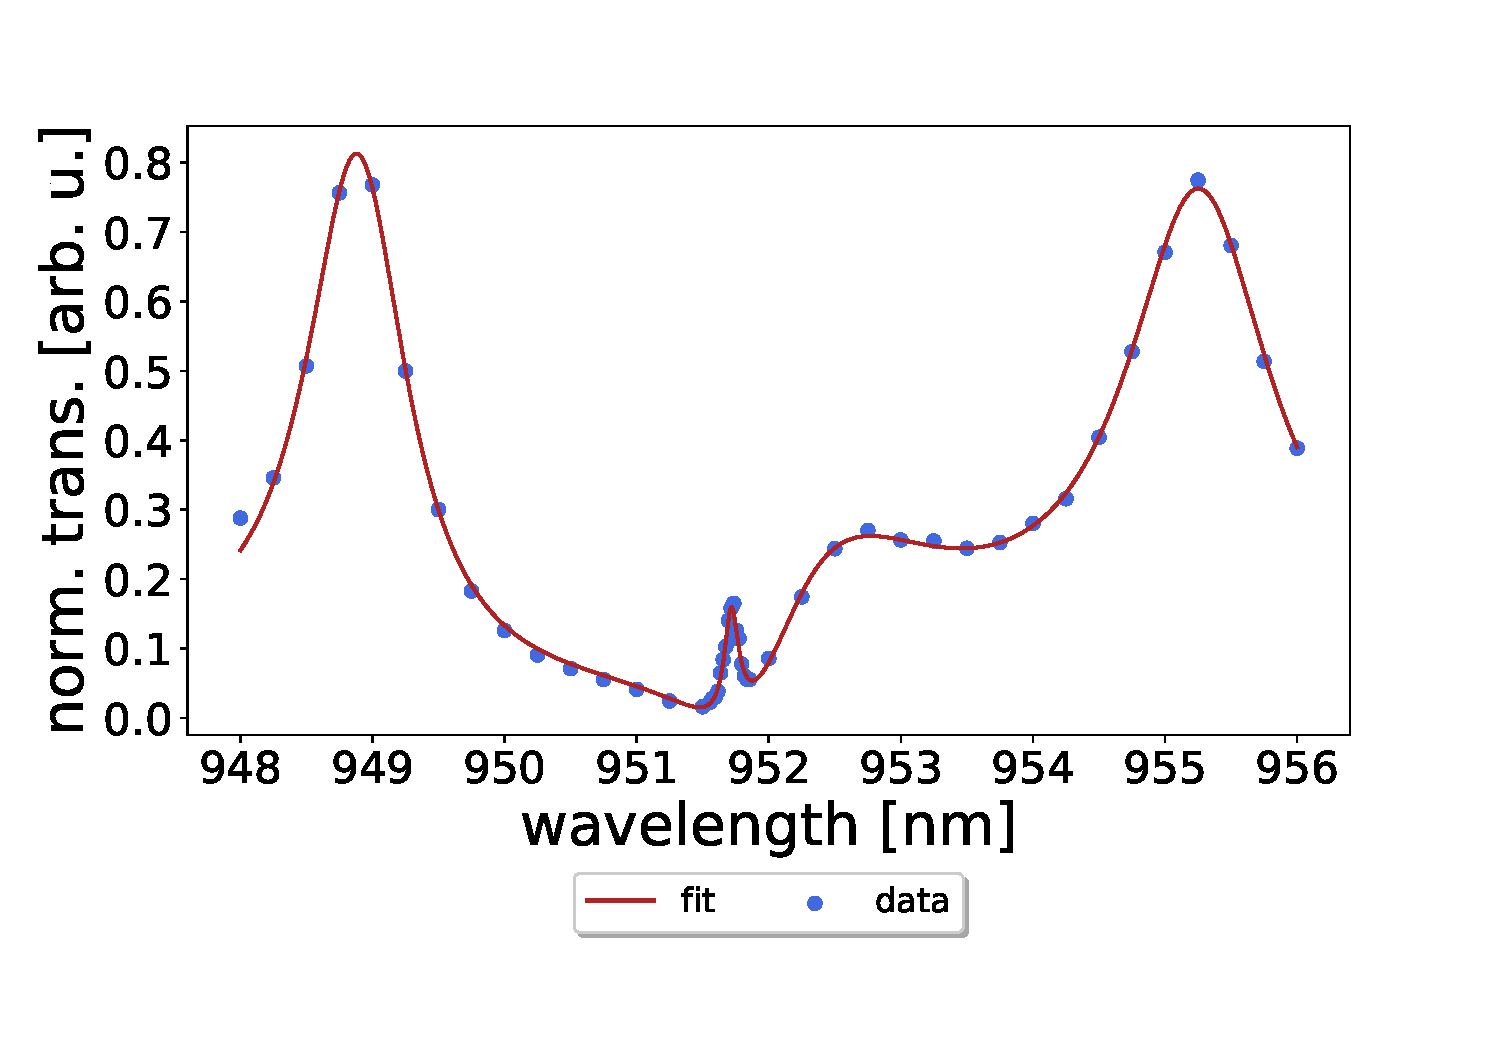
\includegraphics[width=0.7\textwidth]{figures/results/129um_long_scan_fit.pdf}
    \caption{G1: 
    $\lambda$0 =  951.5353433653491 nm 
    $\lambda$1 =  951.6552656404028 nm 
    td =  0.8979113031842125 
    $\gamma \lambda$ =  0.5068297446194285 nm 
    $\alpha$ =  -1.0173070602966957e-06
    G2: 
    $\lambda$0 =  951.8207268469057 nm 
    $\lambda$1 =  951.9411777324733 nm 
    td =  0.6615749475934666 
    $\gamma \lambda$ =  0.5178112810929723 nm 
    $\alpha$ =  9.692094797331468e-07
    cavity length:  139.00222918995942 $\mu$m
    losses:  0.20492009115141496
    }
    \label{fig:129um_long_scan_fit}
\end{figure}

\begin{figure}[h!]
    \centering
    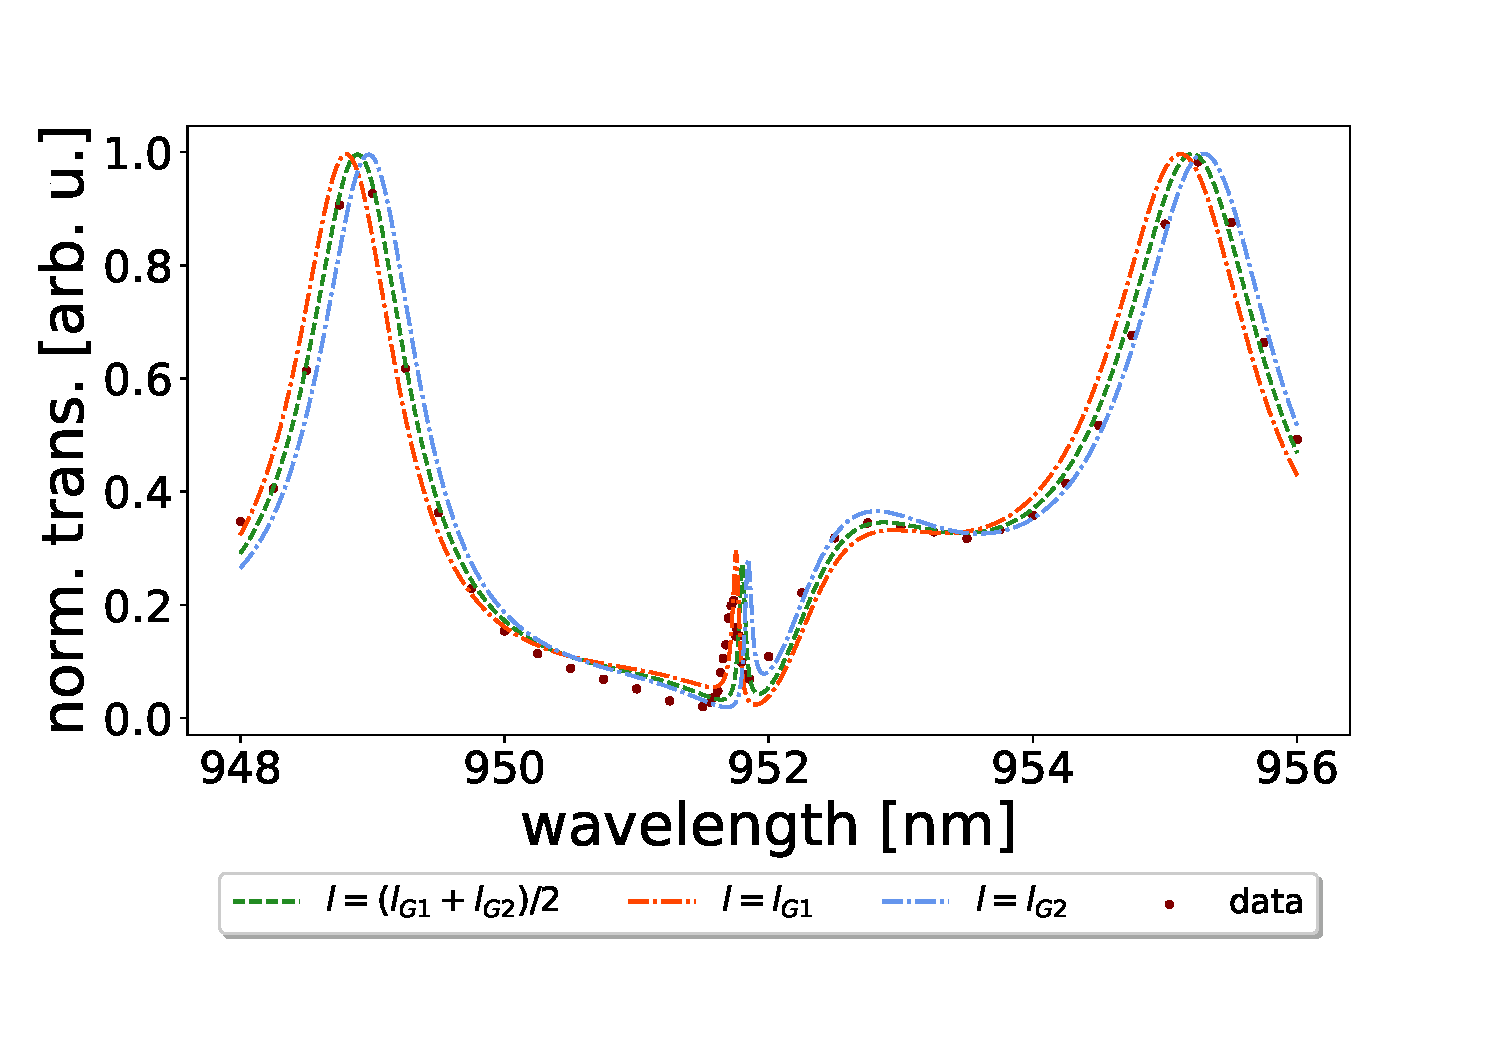
\includegraphics[width=0.7\textwidth]{figures/results/129um_long_scan_sim_comparison.pdf}
    \caption{$l_{G1} = 140.4152 \mu m$, $l_{G2} = 140.4401 \mu m$, $(l_{G1} + l_{G2})/2 = 140.4277 \mu m$}
    \label{fig:129um_long_scan_sim_comparison}
\end{figure}

\begin{figure}[h!]
    \centering
    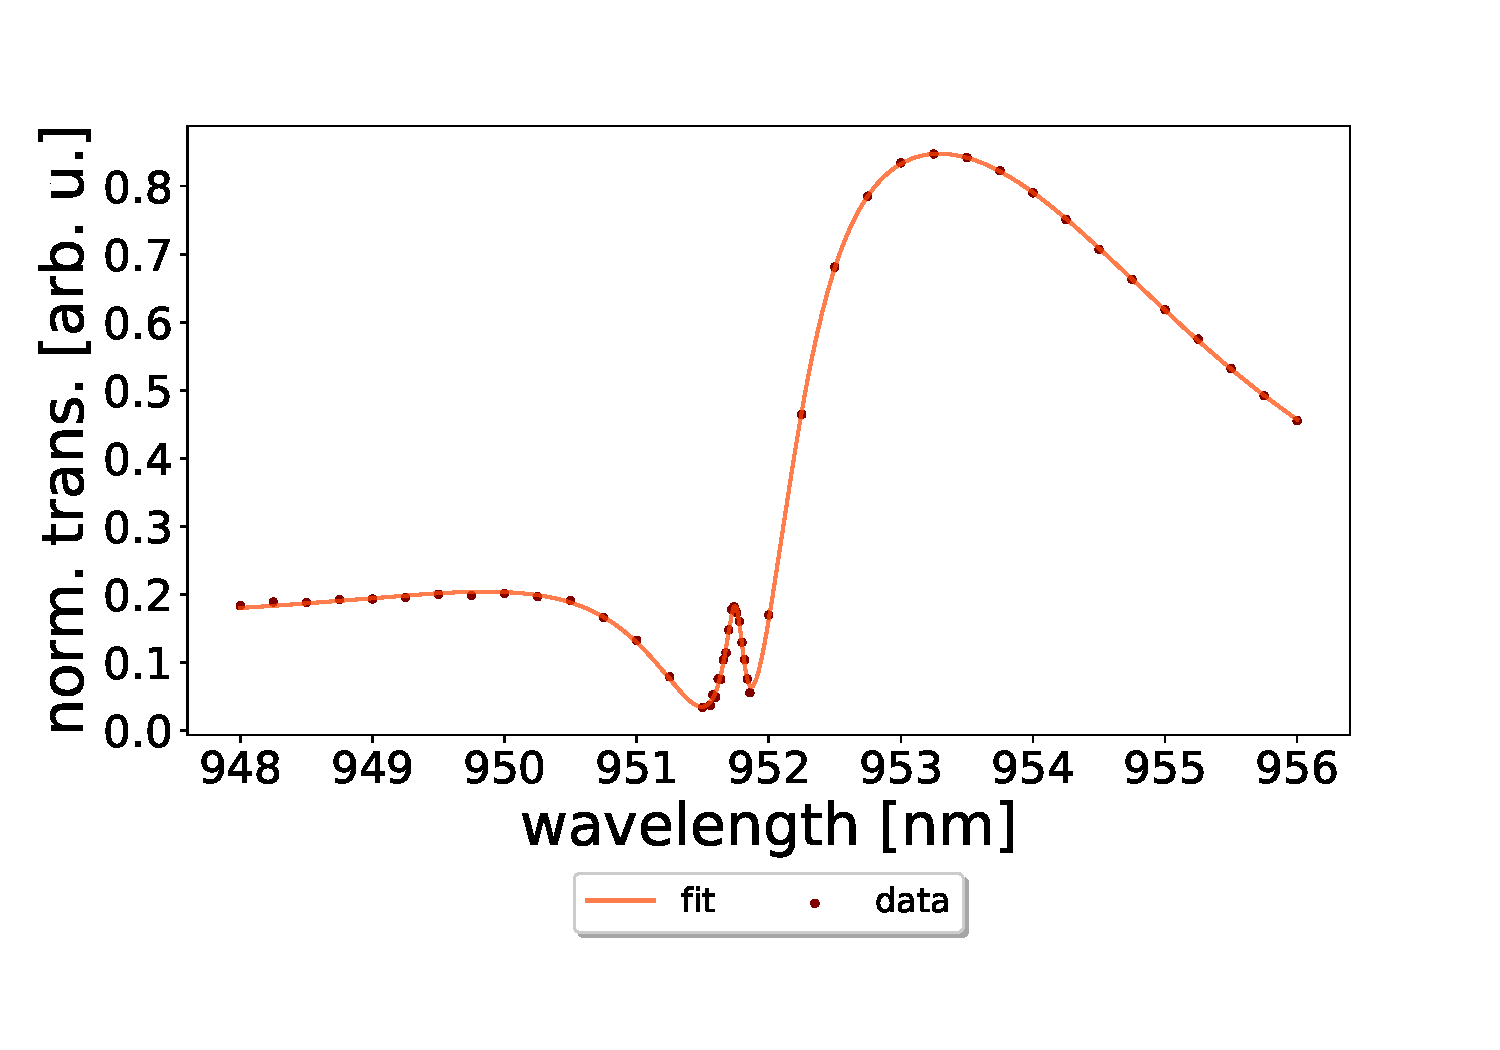
\includegraphics[width=0.7\textwidth]{figures/results/34um_long_scan_fit.pdf}
    \caption{}
    \label{fig:34um_long_scan_fit}
\end{figure}

\begin{figure}[h!]
    \centering
    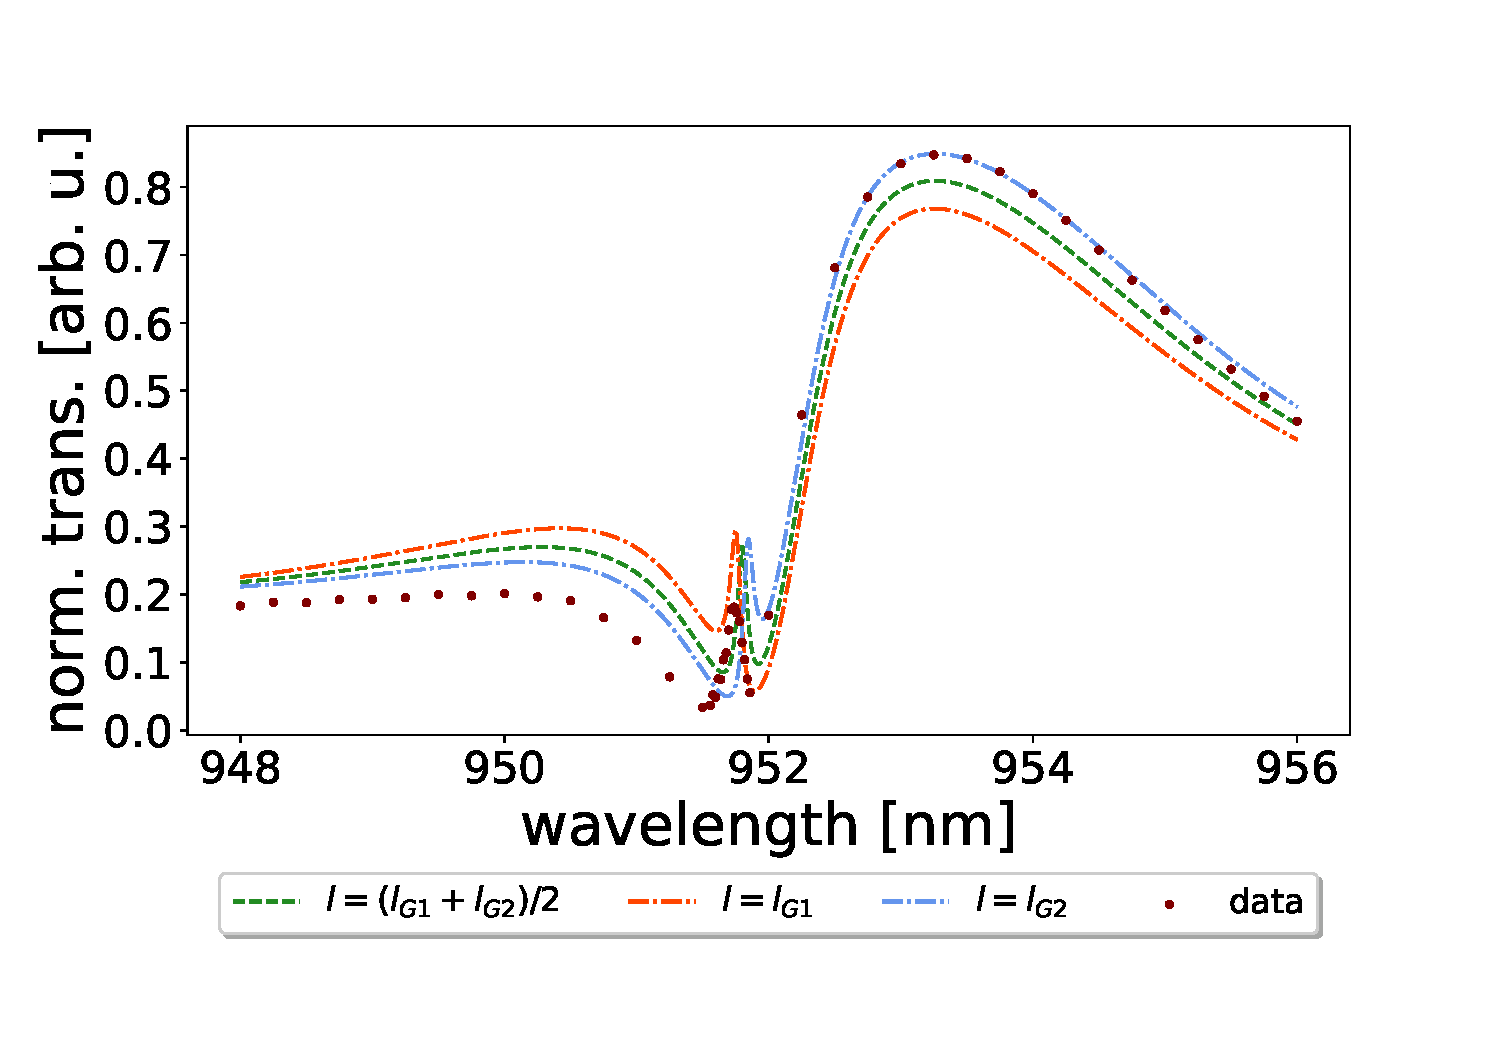
\includegraphics[width=0.7\textwidth]{figures/results/34um_long_scan_sim_comparison.pdf}
    \caption{}
    \label{fig:34um_long_scan_sim_comparison}
\end{figure}

\subsubsection{Double fano off-resonance Fabry-Perot cavity}

Figures:
\begin{itemize}
    \item Off-resonance double fano transmission as a function of wavelength (show that the off resonance transmission goes close to 100 percent for a well-aligned cavity).
\end{itemize}

\subsubsection{The double fano linewidth}

Figures: 
\begin{itemize}
    \item "Semi-short" scan data, fit to the double fano transmission model. 
    \item Short scan data, fit to the Fano function (for measuring linewidth).
    \item Linewidth as a function of cavity length (compare double fano, single fano and broadband cavitites).
\end{itemize}

